\section{Figma Designs}
\label{research:FigmaDesign}
Whilst It is very easy to produce hand drawn diagrams and ideas for my user experience / software design. I searched for a more professional method to produce better visualisations. My search took me to Figma - an industry standard, free to access tool that allows designers to mock up websites, applications and more. While I am by no means a designer I still appreciate many of the tools such as precise element measuring which will enable me transfer my finished designs to in production code more easily

To learn more about Figma I followed this YouTube tutorial \cite{kevinstratvertFigmaTutorialBeginners2024} and then crated these basic designs below (remastering sketches I made for some prior projects):

\begin{figure}[H]
    \centering
    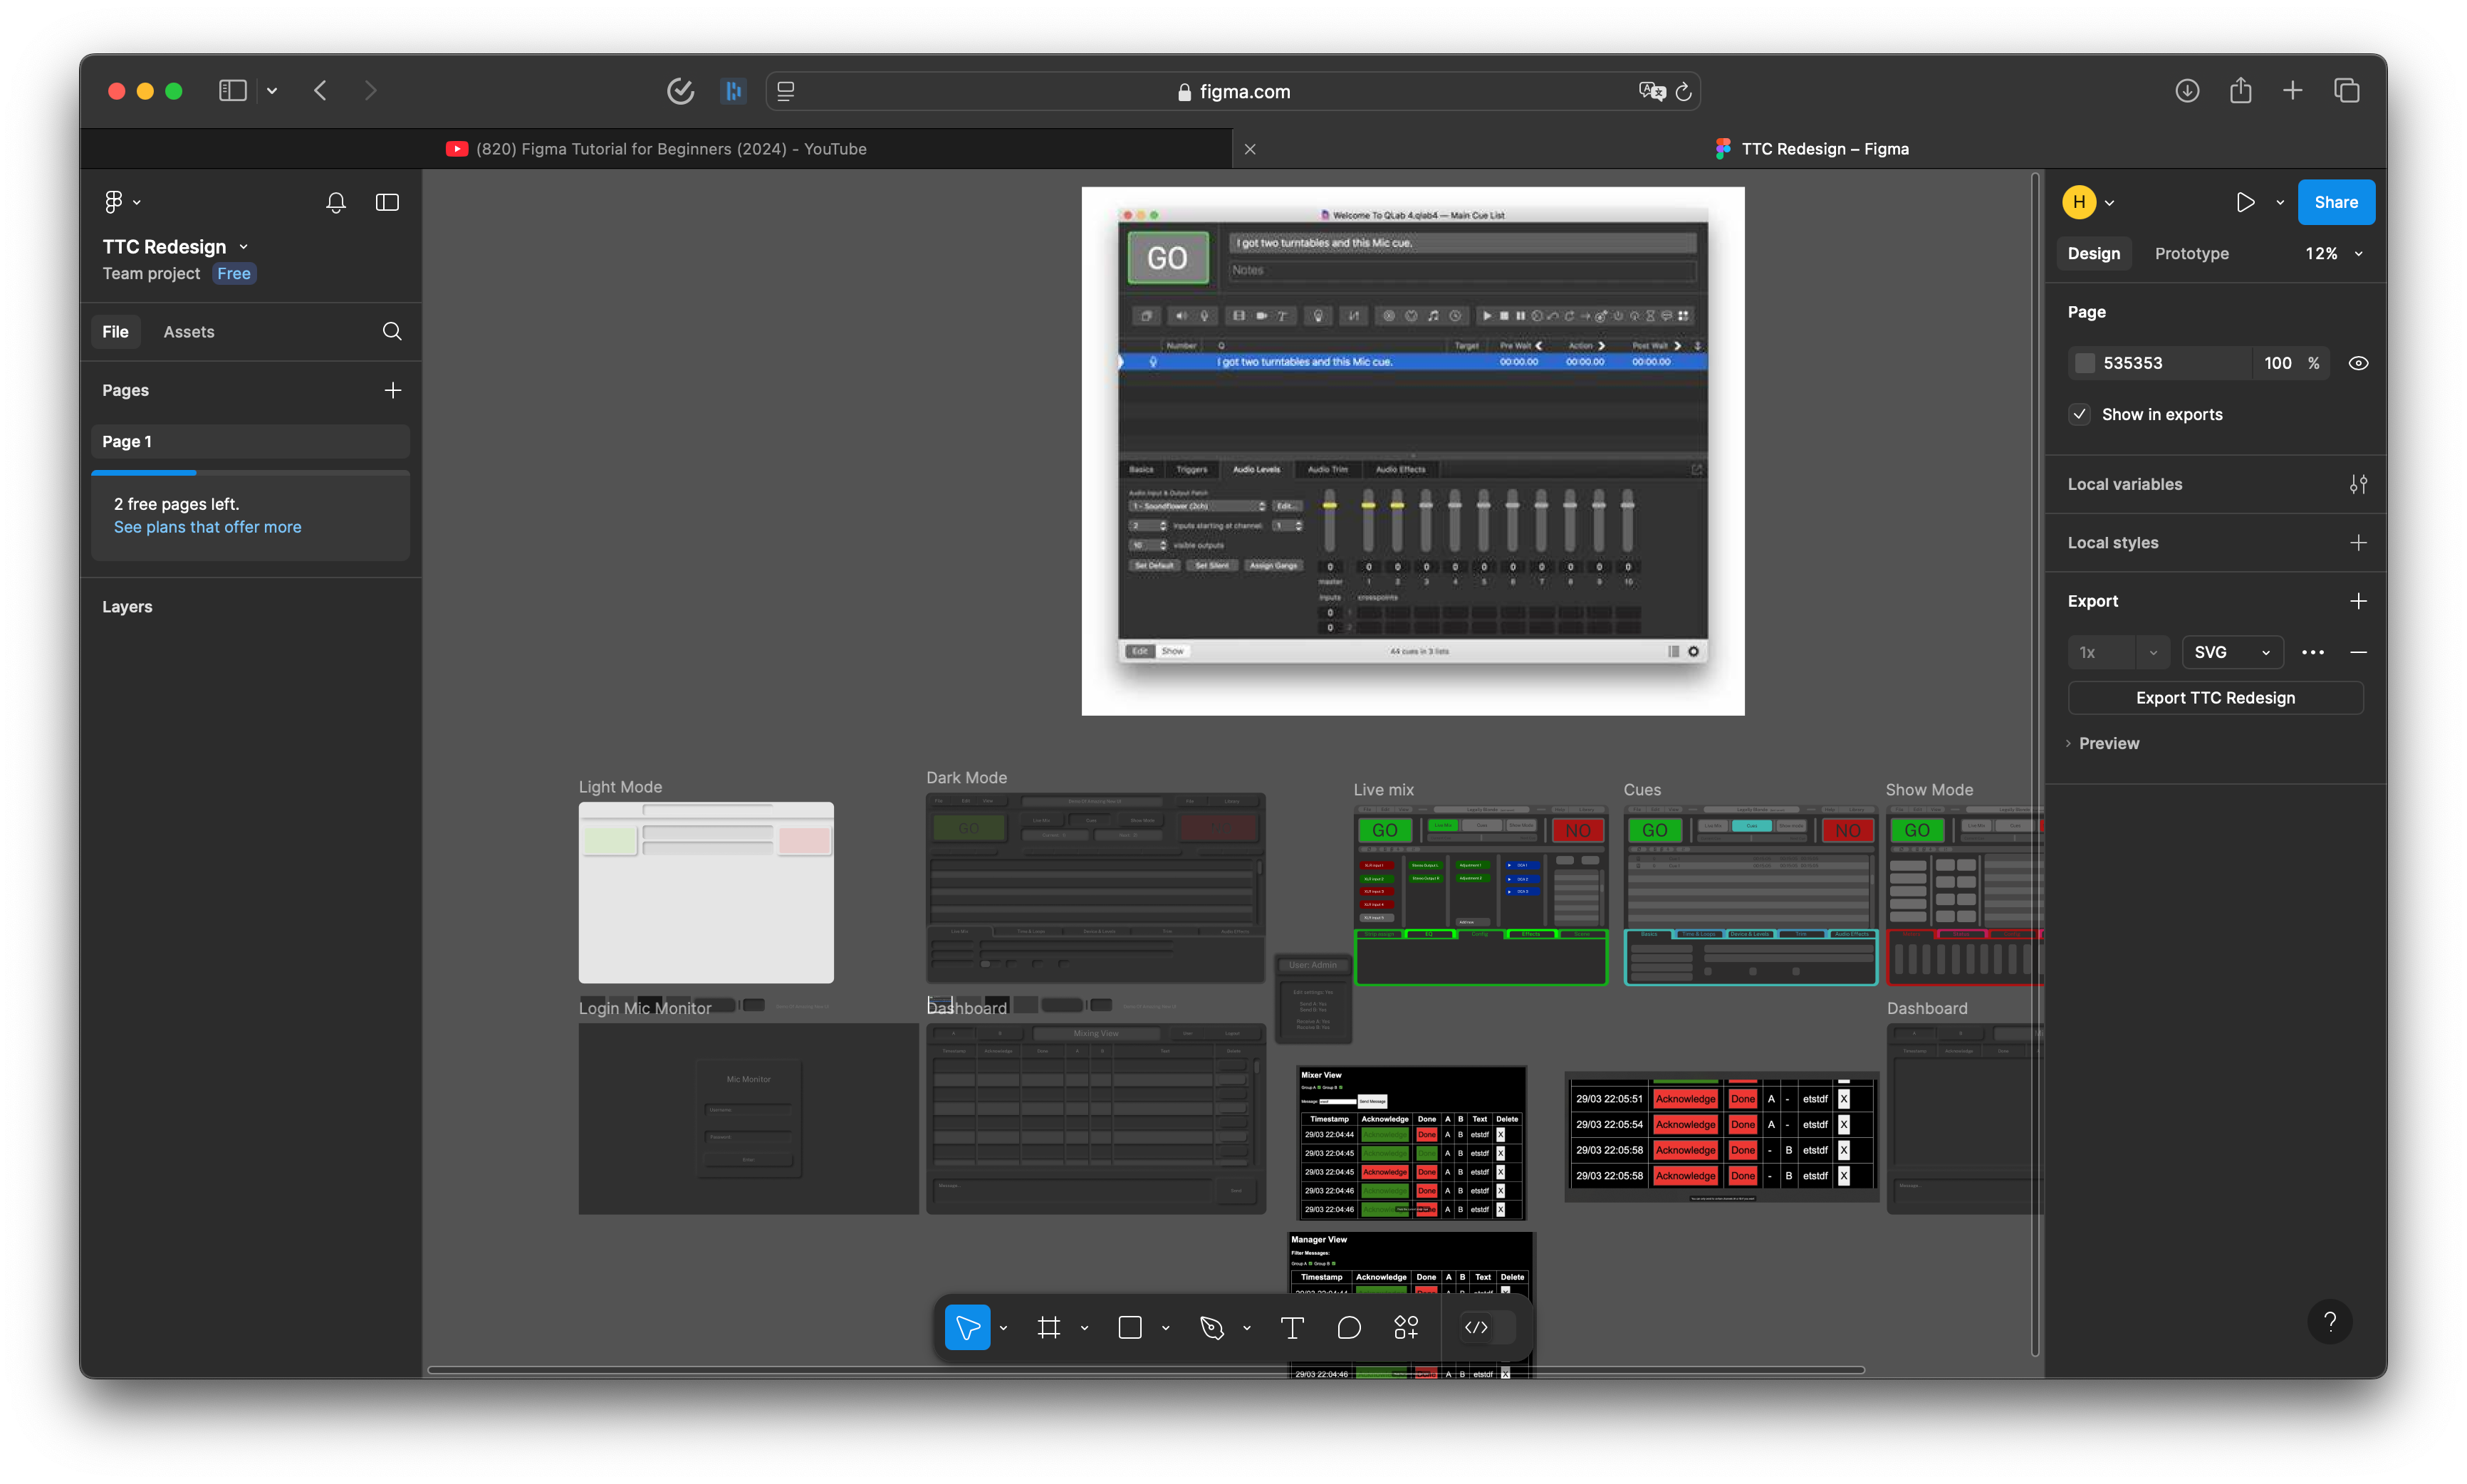
\includegraphics[width=0.8\textwidth]{Research/7_FigmaDesign/media/KewLab.png}
    \caption{Kewlab, a specilised sound effect playback system}
    \label{fig:FigmaDesign1}
\end{figure}

In this design I learnt about element spacing, and clear messaging to users by using colour:

\begin{figure}[H]
    \centering
    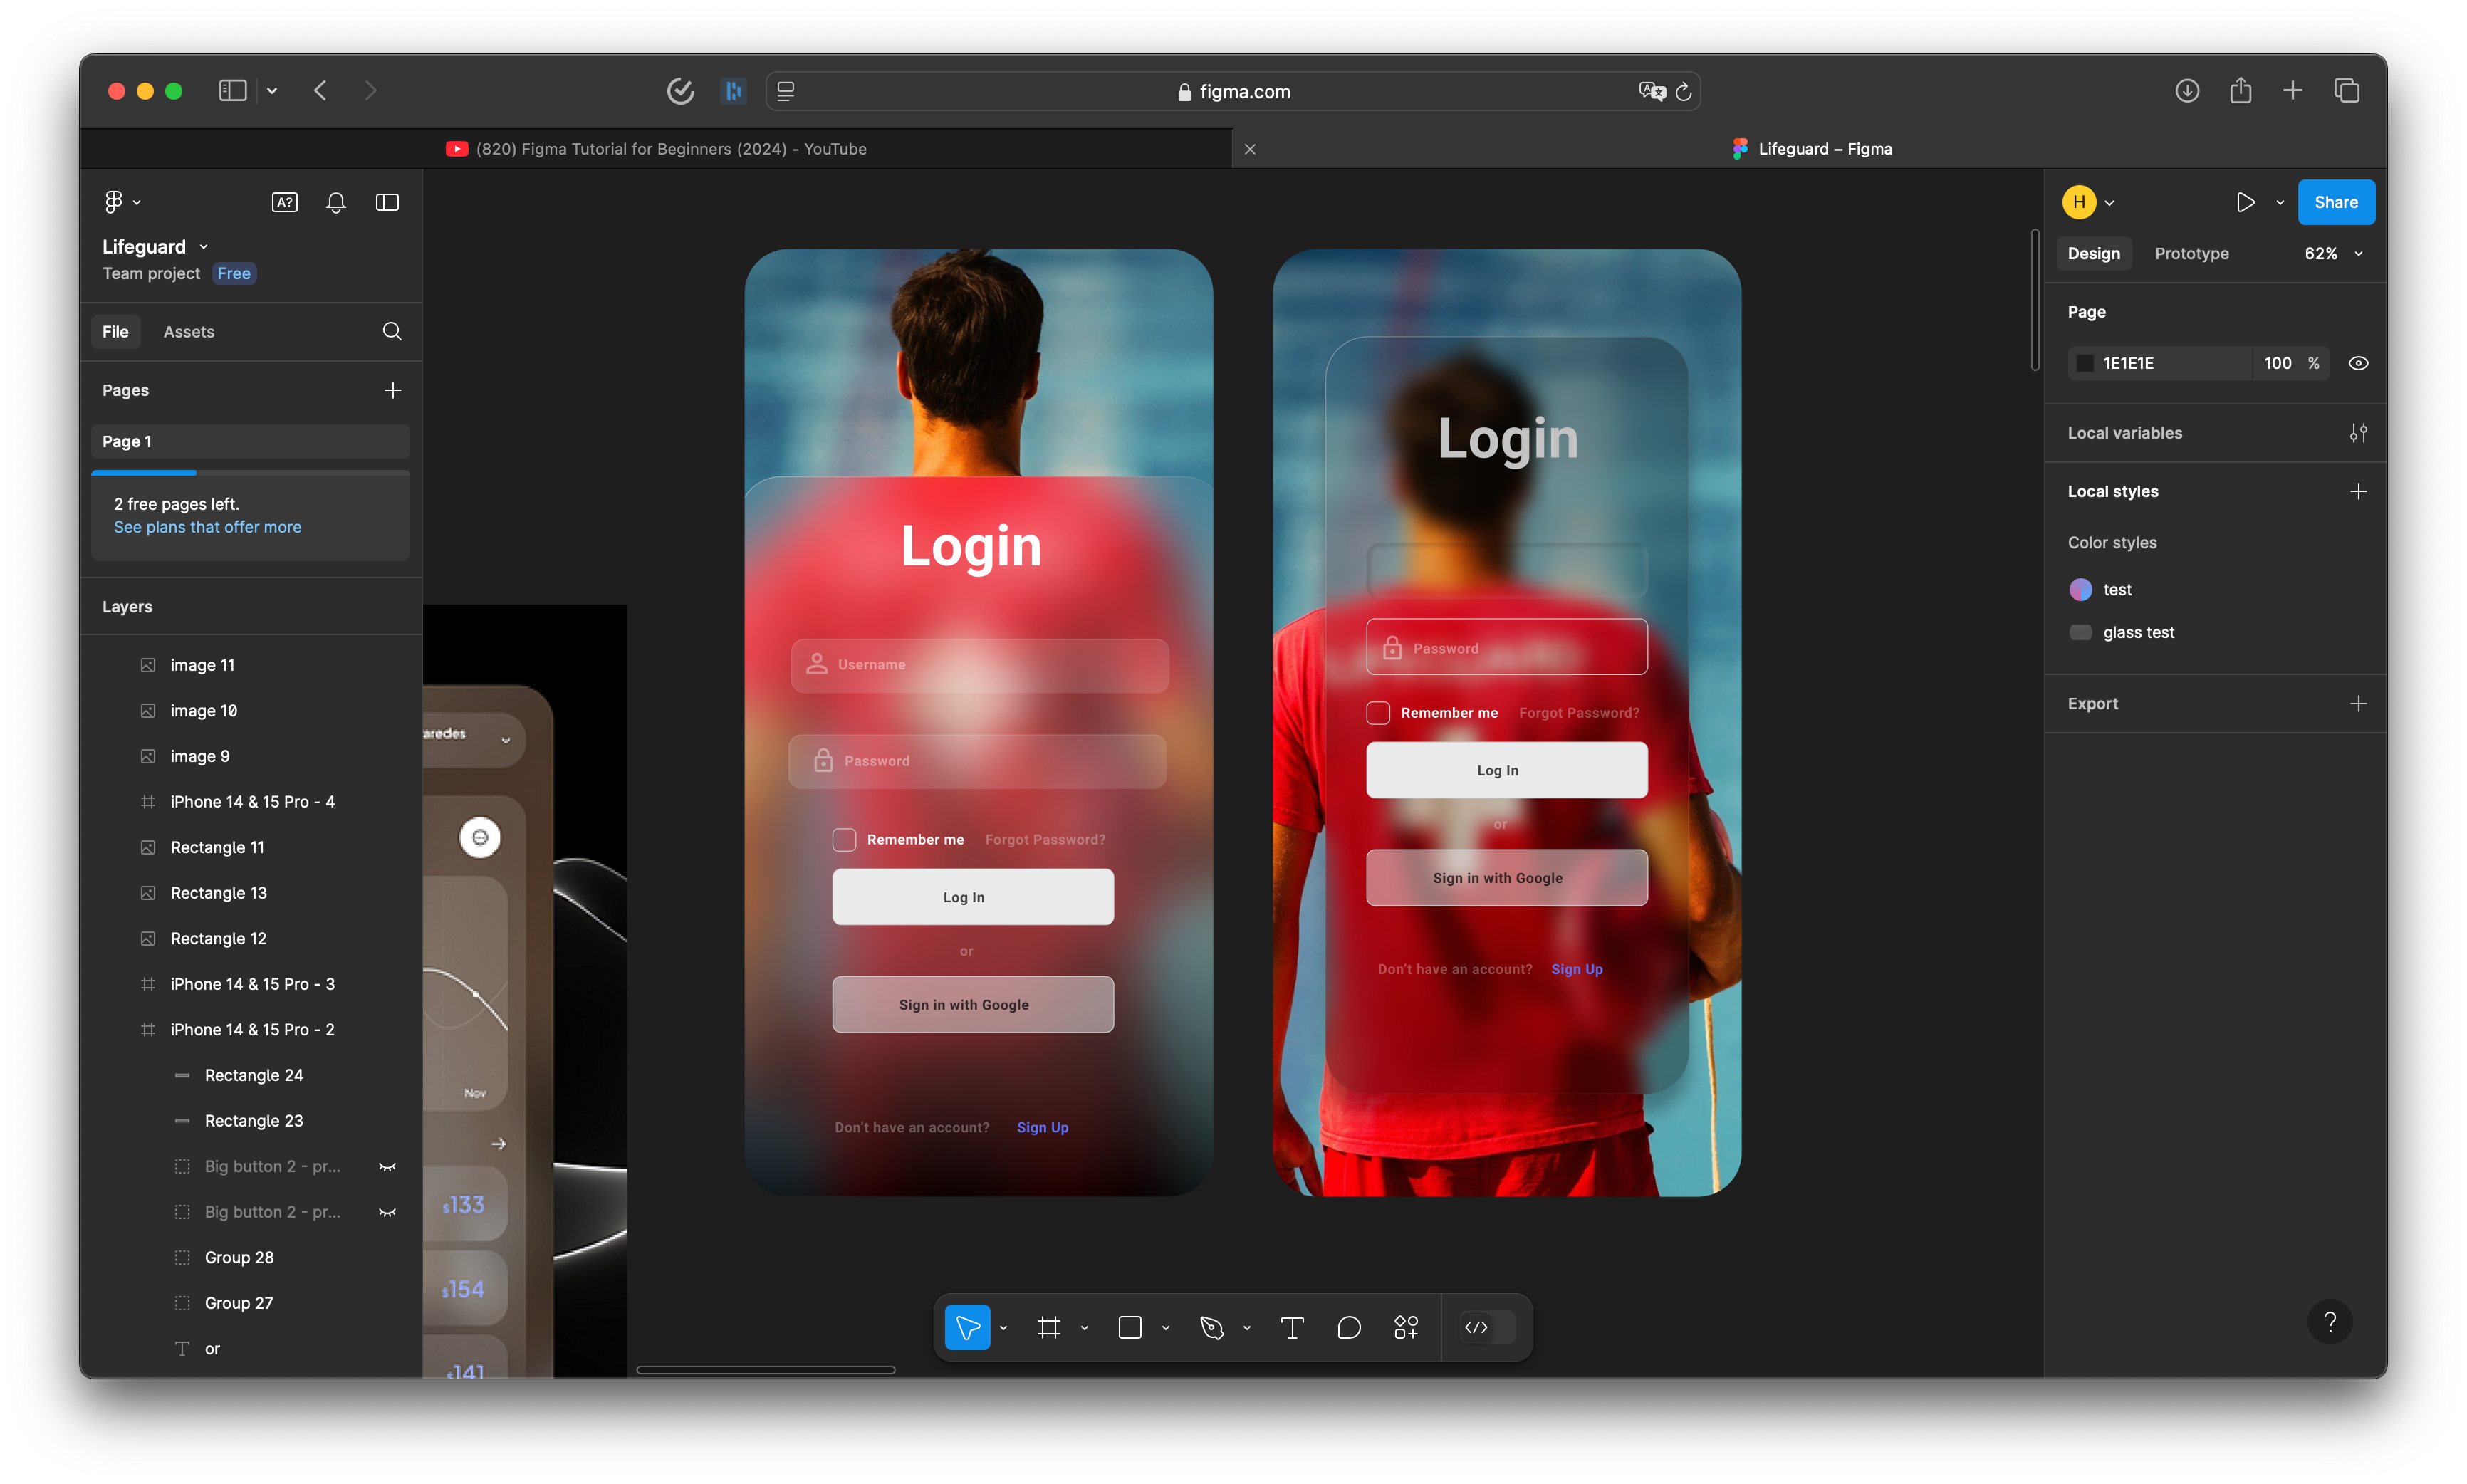
\includegraphics[width=0.8\textwidth]{Research/7_FigmaDesign/media/Lifeguard.png}
    \caption{Lifeguard application, a tool to help lifeguards manage their pool}
    \label{fig:FigmaDesign2}
\end{figure}

In this design I experimented with transparency to integrate corporate branding within an application. I didn't particularly like this implementation of the design but I learnt a lot from it.


\begin{figure}[H]
    \centering
    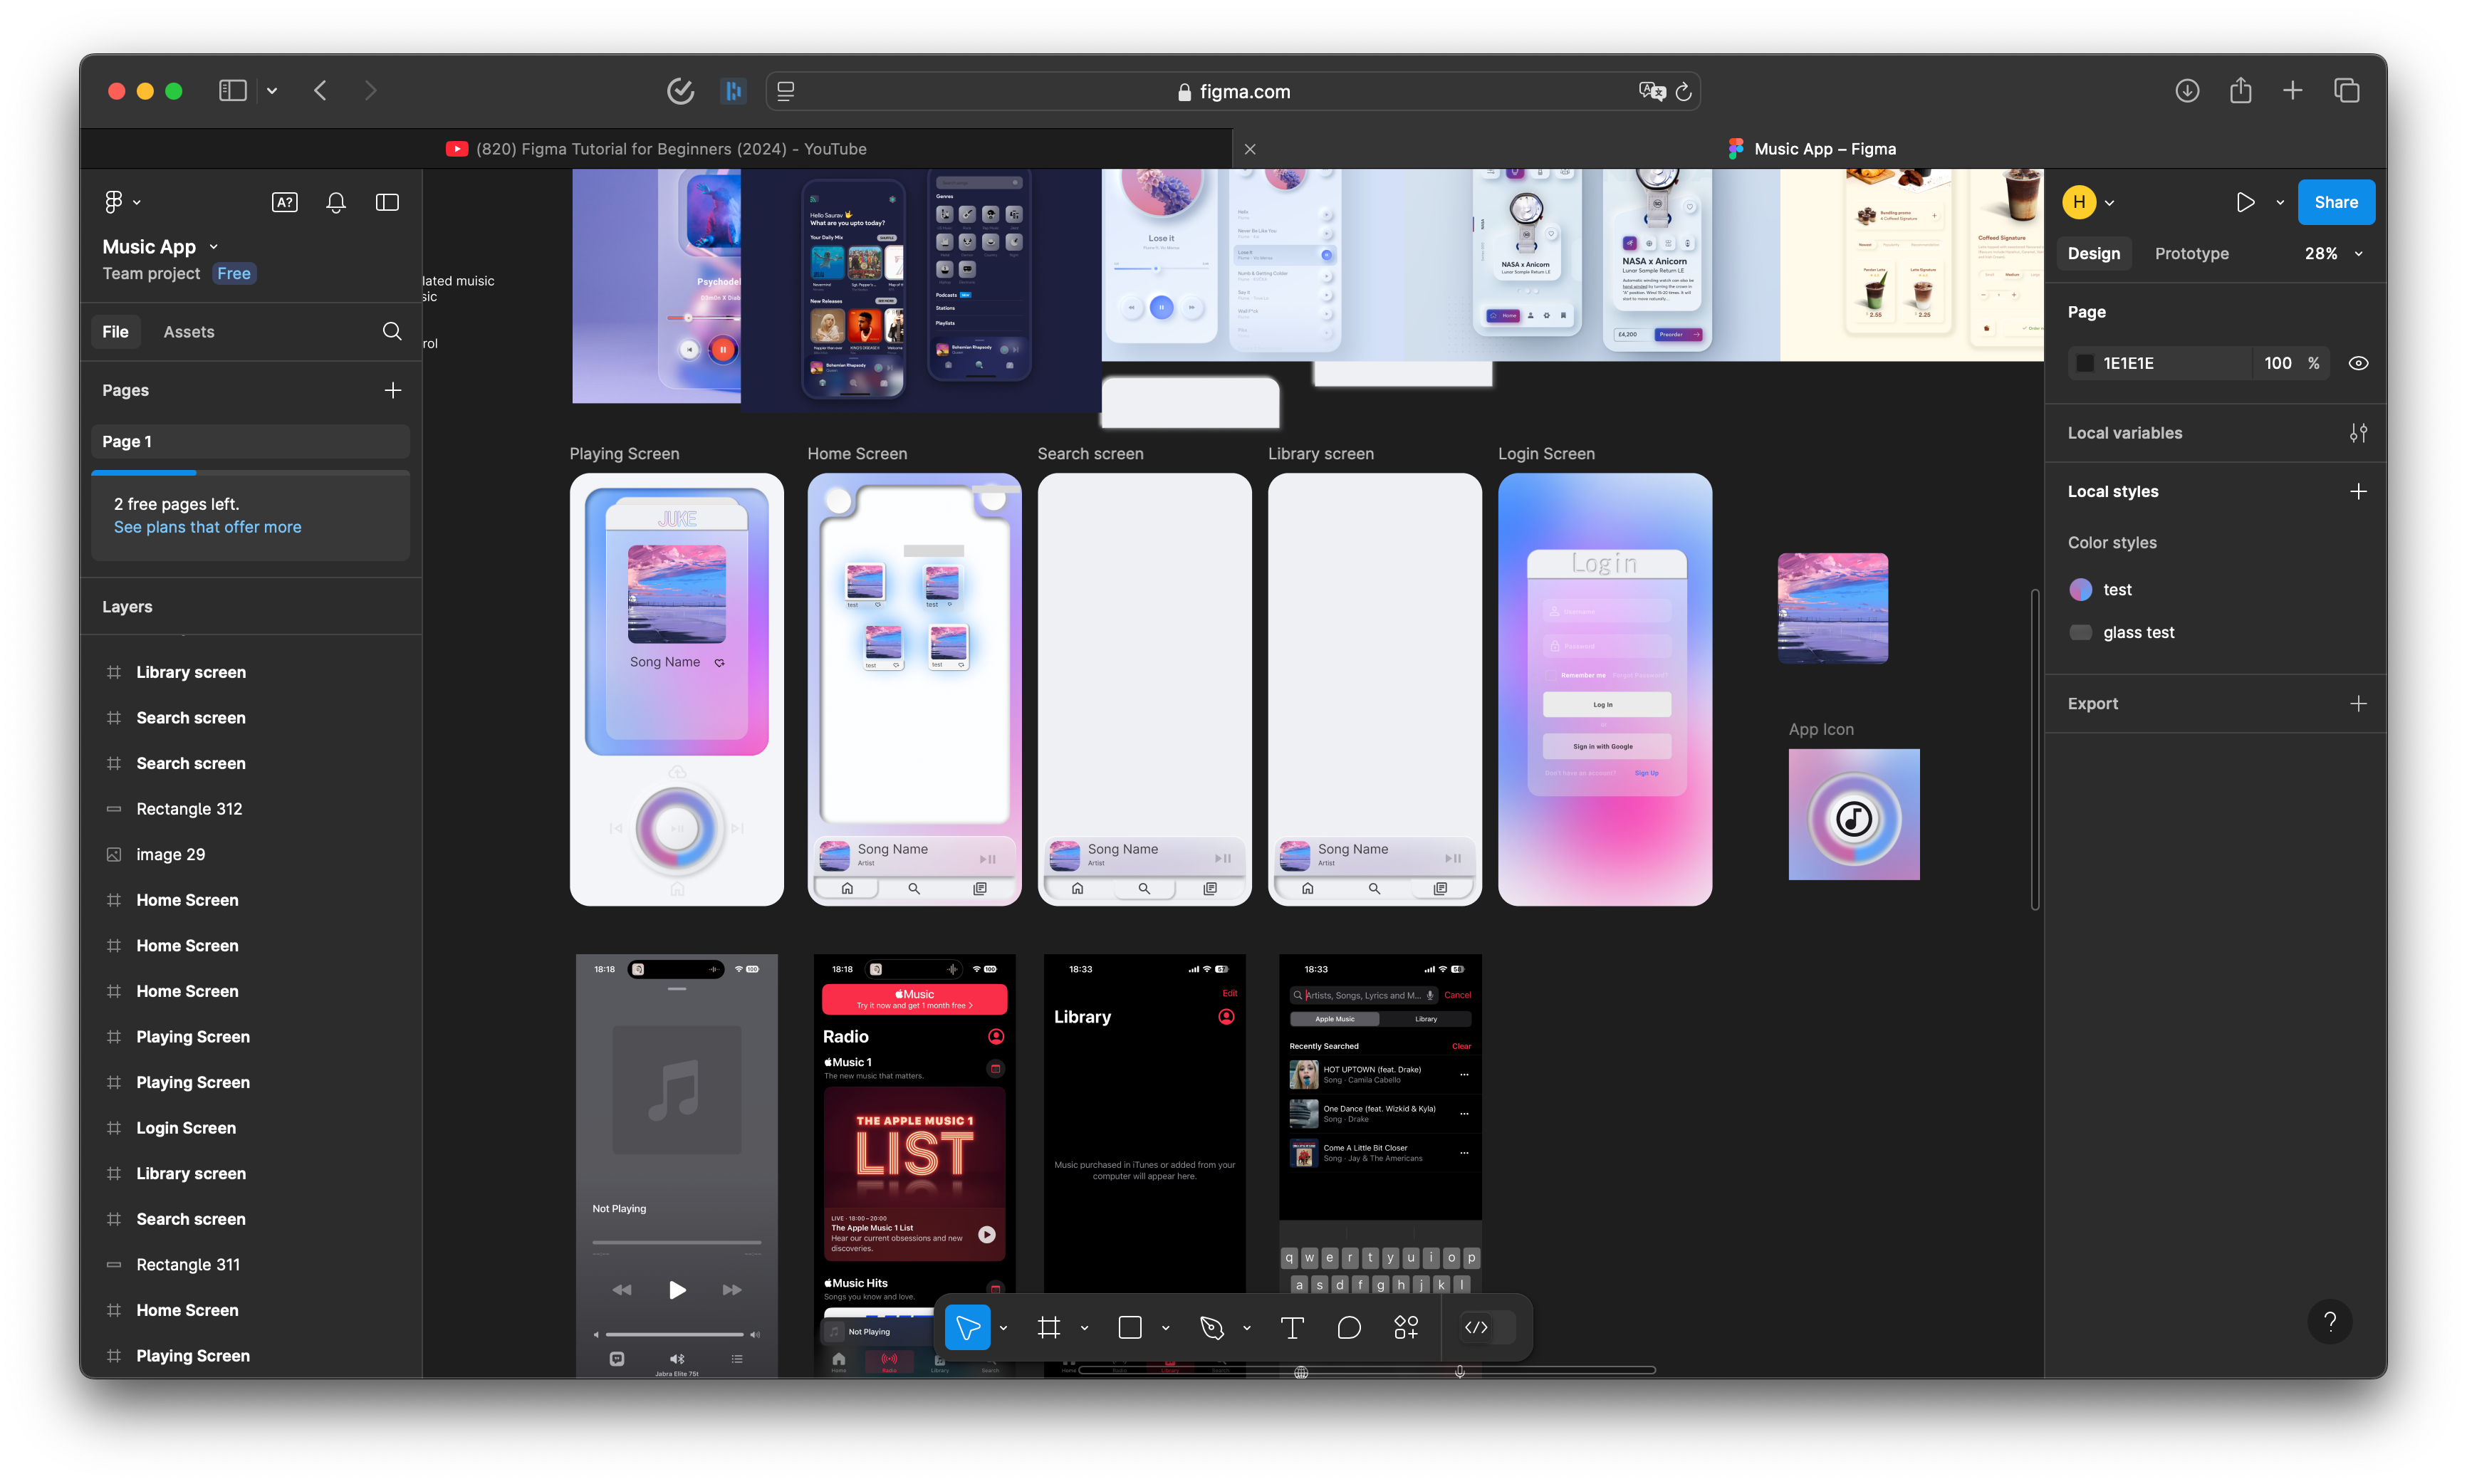
\includegraphics[width=0.8\textwidth]{Research/7_FigmaDesign/media/music.png}
    \caption{Music Playback application}
    \label{fig:FigmaDesign3}
\end{figure}


This design taught me all about creating interfaces for a mobile device and the usability constraints that must be accounted for such as smaller screen sizes, touch targets (as touch used as input not a mouse) and therefore much reduced access to keyboard shortcuts.







